\section{Méthodologies}
Nous présenterons dans cette section l'organisation générale du groupe et les outils qui nous aidé tout au long de ce projet.
On abordera d'abord les outils que nous avons utilisés pour partager 
notre travail le plus efficacement possible.
On présentera ensuite notre manière de gérer la bibliographie
ainsi que les logiciels utilisés pour ne pas perdre les sources visitées.
On détaillera ensuite l'organisation interne du groupe,
plus précisemment le système mis en place pour optimiser la communication
ainsi que la manière dont les tâches ont été réparties tout au long de ce projet.
On décrira finalement les problèmes, difficultés qui
!!!!SONT SURVENUS PARTIE A FAIRE QUAND CODE MARCHERA


\subsection{Outils de travail collaboratif}
Pour des raisons pratiques et esthétiques, nous avons décidé d'écrire
nos rapports en \LaTeX{}.
Il s'agissait donc de trouver la meilleure façon de partager le code source
et de pouvoir contrôler les changements apportés au document.
Une première idée pourrait être d'utiliser ShareLaTeX qui propose une plate-forme
de compilation en ligne ainsi qu'un système de gestion de versions
assez simple à utiliser.
Nous n'avons pas choisi cette solution notamment pour les raisons suivantes.
L'utilisateur doit être connecté dès qu'il veut travailler sur le projet,
le système de compilation est assez lent et l'utilisateur n'est pas libre
d'utiliser son éditeur de texte ou son visualisateur de \textsc{pdf} favori.

Pour palier aux problèmes décrits ci-dessus, le logiciel \texttt{git}
associé à GitHub est une très bonne alternative.
Il permet en effet à chaque membre du groupe de travailler sans être connecté
ainsi que d'utiliser son éditeur et compilateur favori.
Chaque membre travaille donc de son côté en faisant des \emph{commits}
et lorsqu'il juge que son travail est utile pour les autres, 
il \emph{push} sur le serveur.
L'algorithme du fusion, \emph{merge}, permet également de fusionner intelligemment
les lignes d'un fichier qui ont été modifiées par plusieurs membres.
Le dernier point à souligner est que \texttt{git} permet une gestion des branches,
particulièrement pratique lorsqu'on veut développer une partie du projet
sans risquer de créer des erreurs dans le programme principal.

Nous combinons donc ces deux outils pour 
\begin{enumerate}
  \item implémenter le modèle LNAS blé dans la plateforme
  Pygmalion en \textsc{Julia} %(une description plus détaillée de
%  l'objectif attendu pour cette partie est décrite dans la
%  section~\ref{sec:contexte} à la page~\pageref{sec:contexte})
  pour le client dont le code source est sur la plateforme GitLab,
  \item rédiger l'étude documentaire en partageant le code \LaTeX{}
  à l'aide d'un dossier sur 
  GitHub\footnote{\url{https://github.com/jdewasseige/projet-sbt11}}.
\end{enumerate}


\subsection{Gestion de la bibliographie}
Pour la gestion de la bibliographie au sein du document,
nous utilisons le package \texttt{biblatex}.
Celui-ci permet d'écrire l'ensemble de nos références dans un fichier \texttt{.bib}
sous la forme suivante.
\begin{verbatim}
  @online{histoire_mod_plantes,
    title = {Une histoire de la modélisation des plantes},
    author = {Philippe de Reffye and Marc Jaeger 
    and Paul-Henry Cournède},
    url = {https://interstices.info/jcms/c_38032/une-histoire-de-
    la-modelisation-des-plantes},
    year = {2009},
    month = "04",
  }
\end{verbatim}
La mise en page est alors automatique en fonction des informations fournies
et le rendu de l'exemple est présenté ci dessous.
\begin{figure}[h]
  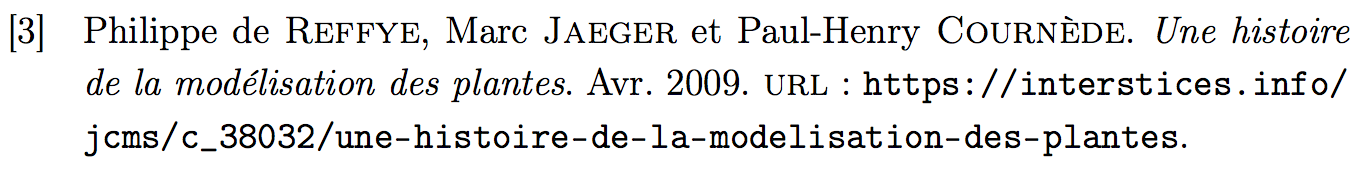
\includegraphics[scale=0.6]{./img/rendu_elem_bib.jpg}
\end{figure}

Cela parait à priori assez lourd d'écrire soi-même toutes les informations
en suivant cette syntaxe mais il existe des logiciels comme Zotero
qui font le travail à notre place.
Les sources trouvées sur Google Scholar peuvent également être exportées
aisément au format \texttt{BibTex}.

\subsection{Organisation et partage des tâches}
Il nous reste un dernier point à décrire, celui de la \emph{communication}
au sein du groupe.
Nous utilisons Slack\footnote{\url{https://slack.com/}} qui est un logiciel
de plus en plus utilisé pour les travaux de groupe ainsi que dans les start-ups.
Il permet d'éviter de devoir alterner entre plusieurs applications comme les mails,
DropBox et Twitter, puisqu'il permet d'être connecté
à celles-ci au sein de l'application.
On peut également créer plusieurs \emph{channels} pour séparer la communication
entre les différentes tâches.
Par exemple dans ce projet nous avons les \emph{channels} suivantes :
\texttt{general}, \texttt{etude-documentaire}, 
\texttt{planning} et \texttt{dev\_plate-forme}.
On trouve aussi un système d'historique et de gestion de fichiers efficace.

L'ensemble des tâches ainsi que leur répartition pendant l'année
est associé au planning \textsc{Gantt} qui se trouve
dans l'Annexe~\ref{ann:planning} à la page~\pageref{ann:planning}.

\subsection{Agenda}

Nos travaux au cours de ce semestre sont présentés dans ce tableau.

IMPOSSIBLE DE METTRE LA PHOTO

%\begin{figure}[h]
%	\begin{center}
%  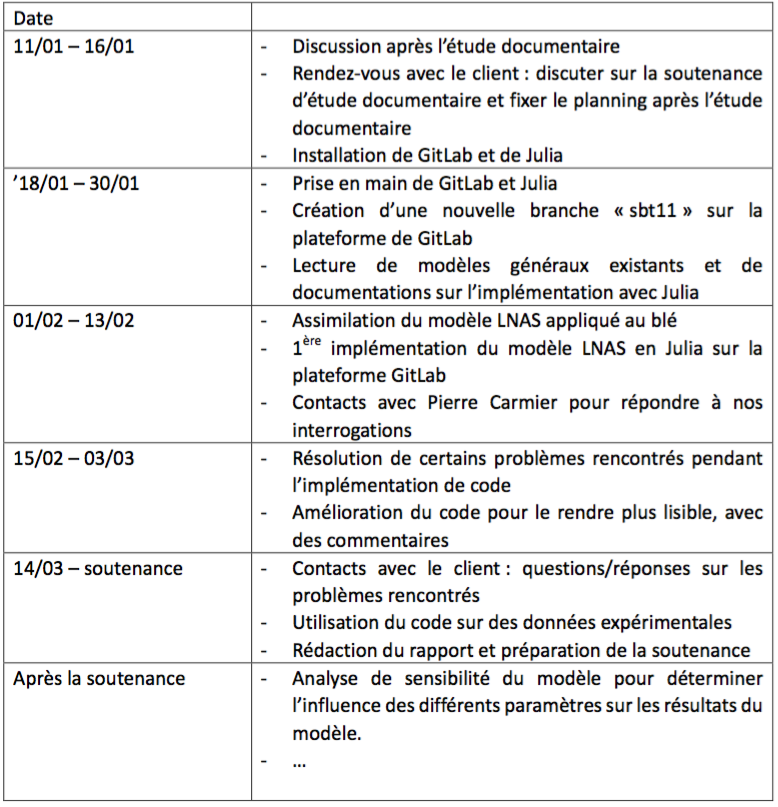
\includegraphics[scale=0.51]{./planning.png}
%  \caption{Agenda de nos travaux au cours du second semestre.}
%  \label{fig:agenda}
%	\end{center}
%\end{figure}

\subsection{Principales difficultés ?????....}


\subsubsection{Difficultés informatiques}

Au cours de ce projet, nous avons été confrontés à de nombreuses difficultés.

Le temps fût une difficulté récurrente. Nous n'étions sans doute pas prêt à gérer de nous-même notre temps. C'est ainsi que nous avons réalisé l'opportunité que constitue ce type de projet. 
Jusqu'à maintenant, nous avions été confrontés la plupart du temps à des questions précises dans des examens, dont l'emploi du temps nous est imposé à l'avance. 
Ici, nous devions de nous même organiser notre temps. 
Nous pourrions nous dédouaner en soulignant l'emploi du temps chargé de nos études à Centrale. 
Mais ce projet est là pour nous rappeler qu'une organisation préalable et une répartition efficace des tâches doivent permettre d'éviter de subir le temps. Et cela s'apprend grâce à des projets comme celui-ci.

\subsubsection{Difficultés informatiques}

Nous avons également été confronté à des problèmes informatiques lors de l'implémentation et de l'utilisation du modèle.
\begin{itemize}
	\item Un bog a empéché au début de nos premières tentatives le lancement de nos programmes. En effet, les chercheurs
du laboratoire MAS qui ont développé la plateforme utilisait les fonctions directement sur leur répertoire, alors que nous devions nous y relier. Un bog, au niveau du chemin, bloquait nos programmes. Il a donc fallu détecter l'origine de ce bog avant de pouvoir commencer à utiliser nos programmes. 
	
	\item De plus, des erreurs classiques sur notre implémentation empéchait également le bon déroulement de nos utilisations du modèle : fautes de frappe...

\end{itemize}
\subsubsection{Difficultés théoriques}
Enfin, certaines formules du document qui décrivait de manière théorique le modèle LNAS appliqué au blé conduisait à des valeurs pas cohérentes : 
Dans un premeir temps la croissance de la plante était trop faible. Il a fallu changer les fonctions log-normales dans les fonctions d'allocation, de remobilisation et de sénescence.
La formule donnée utilisait une définition différente de l'écart type que la formule qui correspondait aux paramètres que Pierre Carmier nous avait fournis. 
Une fois ceci corrigé, nous obtenions cette fois des récoltes beaucoup trop élevées, plus de 3000 en grains et environ 16 en LAI, alors que les valeurs attendues sont respectivement d'environ 1000 et entre 5 et 6.
Cela était dû à l'abscence de prise en compte dans le modèle théorique du temsp de montaison, temps à partir duquel la tige commence à croître de manière très rapide. Car à partir de ce temps, l'essentiel de la biomasse est allouée à la tige.
Ainsi, après allocation à la graine (celle-ci étant nulle au départ puis tendant vers 1 très rapidement à maturité de la plante), on répartissait par défaut (sans stress hydrique ou thermique) la biomasse produite aux compartiments restants (tige, racines, et feuilles) de façon égale. Ceci est peu réaliste. Nous avons donc introduit un temps de montaison, tout d'abord de manière assez abrupte. Il s'agit de ne rien allouer à la tige au départ, puis de lui en allouer de plus en plus. Nous nous sommes contenté de décrire deux régimes, un régime pré montaison et un post, avec une transition instantanée. Plus tard nous comptons faire une transition progressive avec une loi lognormale et rentrer ses paramètres dans le modèle.
Cela permis d'avoir des valeurs réalistes pour le LAI et la quantité de grain est descendu à 2500.
Enfin, la trop grande quantité de grain, dernière grosse incohérence qu'il restait était du au fait que dans le modèle qu'on nous a donné, au moment vers la maturité de la plante, toute la biomasse de la tige était réaloouée au grain ce qui n'est pas réaliste. Nous avons donc rajouté un comporatiment "tige jaune", une sénessence de la tige en tige jaune de façon à ce que une partie de la biomasse de la tige ne soit jamais allouée au grain.
Après l'ajout de ce compartiment au modèle nous avons obtenu des valeurs de grain finales autour de 2000, ce qui était encore trop. 
Nous pensons à regarder encore si le modèle peut améliorer, mais surtout à commencer à jouer sur les paramètres (cf perspectives)
 
 la biomasse totale du champ continuait de grandir sans culminer. 
Les connaissances de Pierre Carmier sur les modèles de croissance des plantes nous ont permis de savoir ce qui était cohérent dans nos résultats et ce qui ne l'était pas. 
Nous avons donc avec l'aide de notre client ajuster les formules que nous utilisions :  





